\documentclass[a4paper]{article}

\usepackage[pdftex]{graphicx}
\usepackage[margin=3cm]{geometry}
\usepackage{verbatim,moreverb,amssymb,amsmath}


\newcounter{question}
\newcommand{\question}[1]{\refstepcounter{question}\section*{Question~\thequestion~~~\small\emph{(#1)}}}
\renewcommand*\thequestion{\arabic{question}}


\begin{document}

\pagestyle{empty}
\thispagestyle{empty}



\noindent
\begin{minipage}{\columnwidth}
  \centering
  \Large
  DA4002 (HT11) Halmstad University\\
  Introduction to Algorithms, Data Structures, and Problem Solving\\[3\baselineskip]
  \Huge
  Written Exam\\
  \Large
  Tuesday, October 30, 2012\\[2\baselineskip]
  Examiner: Roland Philippsen
\end{minipage}

\vfill

\noindent
\begin{center}
\fbox{
  \begin{minipage}{0.8\columnwidth}
    \textbf{Student Name:}\\[3\baselineskip]
  \end{minipage}
}
\end{center}

\vfill



\section*{Rules}

Aside from the obvious rules of conduct exams (e.g.\ no chatting):

\begin{itemize}
\item
  \textbf{No computing devices} (laptops, phones, calculators, \emph{etc}).
\item
  \textbf{No books or printouts} except for non-electronic dictionaries.
\item
  \textbf{Allowed hand-written notes}: two sheets of A4 paper (front and back).
\end{itemize}



\section*{General Guidelines}

\begin{itemize}
\item
  \textbf{Read carefully} and pace yourself.
  You can solve the problems in any order you want, but later problems may be easier to solve after you have answered the preceding questions.
\item
  \textbf{Write clearly} and draw clear diagrams.
  If you need to correct a mistake, then cleanly cross out the wrong answer and clearly indicate where the correction can be found.
\item
  \textbf{Indicate the question number} for each of your answers.
  If a question has sub-questions, indicate the sub-question number after the main question number, separated by a dot.
  For example, question 3 has 4 sub-questions, and their answers should be numbered 3.1, 3.2, 3.3, and 3.4.
\end{itemize}



\pagebreak
\pagestyle{plain}
\thispagestyle{plain}
\setcounter{page}{1}



\question{6 points}

Below are three diagrams \textbf{(1)}, \textbf{(2)}, and \textbf{(3)}.
Each of them shows the result of inserting the values $\{5, -2, -3, 1, 9, 6\}$ into a different type of data structure.
Beside the diagrams are three data structure declarations \textbf{(A)}, \textbf{(B)}, \textbf{(C)}.
Each of them corresponds to one of the diagrams.
On the next page, there are three different implementations of an \textbf{\texttt{insert}} function.
They are labelled \textbf{(D)}, \textbf{(E)}, \textbf{(F)}.
Each implementation is for a different type of data structure.

\begin{enumerate}
\item
  Fill in the table at the bottom of this page.
  For each of the diagrams
  \begin{itemize}
  \item
    choose the corresponding declaration (from this page),
  \item
    choose the corresponding implementation (from the next page),
  \item
    and write down the name of the data structure.
  \end{itemize}
\item
  For each of these data structures, write code that iterates over all the items and prints their value.
  You can use pseudo-code or C code, or plain English.
\end{enumerate}

\vfill

\noindent
\begin{minipage}{0.4\columnwidth}
  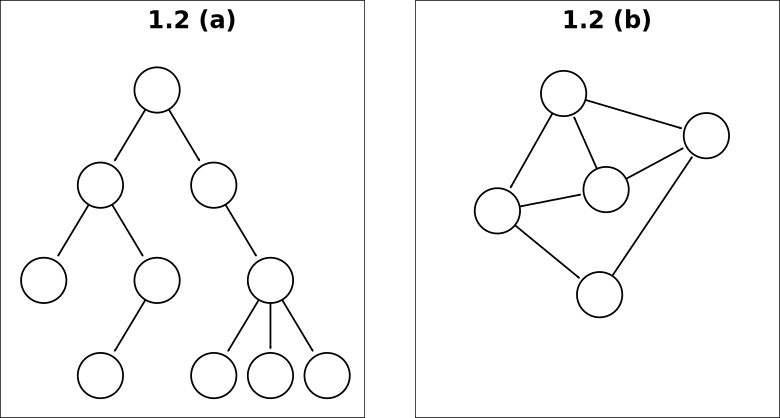
\includegraphics[width=\columnwidth]{q1.pdf}
\end{minipage}\hfill
\begin{minipage}{0.5\columnwidth}
  \small
  \fbox{%
    \begin{minipage}{\columnwidth}
      \hfill declaration \textbf{(A)}
      \verbatimtabinput{clist-decl.txt}
  \end{minipage}}
  \fbox{%
    \begin{minipage}{\columnwidth}
      \hfill declaration \textbf{(B)}
      \verbatimtabinput{minheap-decl.txt}
  \end{minipage}}
  \fbox{%
    \begin{minipage}{\columnwidth}
      \hfill declaration \textbf{(C)}
      \verbatimtabinput{bstree-decl.txt}
  \end{minipage}}
\end{minipage}

\vfill

\begin{center}
  \begin{tabular}{|c|p{0.2\columnwidth}|p{0.2\columnwidth}|p{0.5\columnwidth}|}
    \hline
            & declaration  & implementation & \\
    diagram & (A, B, or C) & (D, E, or F)   & data structure name \\
    \hline
    &&&\\
    \textbf{(1)} & & & \\
    &&&\\
    \hline
    &&&\\
    \textbf{(2)} & & & \\
    &&&\\
    \hline
    &&&\\
    \textbf{(3)} & & & \\
    &&&\\
    \hline
  \end{tabular}
\end{center}


\clearpage

\subsection*{Implementations for Question 1}

\noindent
\fbox{%
  \begin{minipage}{\columnwidth}
    \hfill implementation \textbf{(D)}
    \footnotesize
    \verbatimtabinput{minheap-insert.txt}
\end{minipage}}

\noindent
\fbox{%
  \begin{minipage}{\columnwidth}
    \hfill implementation \textbf{(E)}
    \footnotesize
    \verbatimtabinput{bstree-insert.txt}
\end{minipage}}

\noindent
\fbox{%
  \begin{minipage}{\columnwidth}
    \hfill implementation \textbf{(F)}
    \footnotesize
    \verbatimtabinput{clist-insert.txt}
\end{minipage}}


\clearpage

\question{4 points}



\clearpage

\question{4 points}




\clearpage

\question{6 points}


\clearpage

\question{5 points}



\end{document}
